\documentclass[11pt]{scrartcl}
\usepackage[utf8]{inputenc}
\usepackage{evank}


%% insert title here
\newcommand{\titlee}{Mock $F=ma$ Exam}
\parindent 0 pt

\title{\titlee}
\author{Cambridge Physics Academy}
\date{2023-2024}

\newcommand{\cor}{\textcolor{red}{$\leftarrow$ \textbf{CORRECT}}}

\begin{document}

\thispagestyle{empty}
\begin{center}
    
    
    \Huge \textbf{\textsf{\titlee}}

    \large \theauthor
\end{center}

\begin{prob}
    Alice kicks a soccer ball at a wall at speed $v$ from a distance $L$ away from the wall. The ball bounces elastically off of the wall and lands a distance $L$ behind her. What is the minimum kicking speed $v$ necessary for this to occur?
    \begin{enumerate}[label = (\Alph*)]
\item $\sqrt{gL}$
\item $\sqrt{3gL/2}$
\item $\sqrt{2gL}$
\item $\sqrt{3gL}$ \textcolor{red}{$\leftarrow$ \textbf{CORRECT}}
\item $\sqrt{6gL}$
\end{enumerate}
\end{prob}
\begin{sol}
    The wall just acts as a mirror, so the problem is essentially finding the minimum speed to reach a distance $3L$. The distance formula follows $d=v^2\sin2\theta/g$, and setting $\sin 2\theta=1$ yields $v=\sqrt{3gL}$.
\end{sol}


\begin{prob}
    Ben is playing with a hammer. The hammer is composed of a rod of mass $M$ and length $l$ and a head, which you can treat as a point mass, of mass $m$. He spins it about the hammer's center of mass with angular velocity $\omega$. What is the ratio of the tangential speed of the handle's end to the tangential speed of the hammer's head?
    \begin{center}
        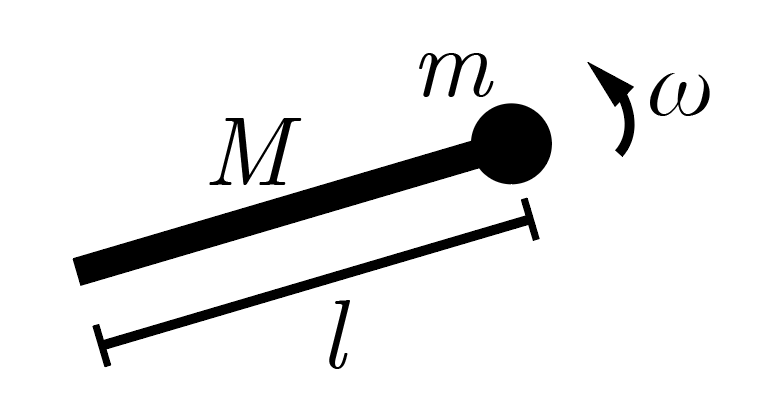
\includegraphics[width=5cm]{hammerr.png}
    \end{center}
    \begin{choices}
        \item $\frac{M+m}{M}$
        \item $\frac{M + 2m}{M}$ \cor
        \item $\frac{M+m}{2M}$
        \item $\frac{2M+m}{2M}$
        \item $\frac{2M+m}{M}$
    \end{choices}
\end{prob}
\begin{sol}
    Since the hammer is spinning about its COM, we just want to find the ratio of the distance of the end of the hammer to the COM and the distance of the head to the COM. The center of mass is a distance
    $$x = \frac{m}{M+m}\frac{l}{2}$$
    from the COM of the handle, which means that the COM is the following distances from the two ends:
    $$x_{\text{end}} = \frac l2 + \frac m{M+m} \frac l2 = \frac{M+2m}{M+m}\frac l2, x_{\text{head}} = \frac l2 - \frac{m}{M+m} \frac l2 = \frac{M}{M+m} \frac l2.$$
    Thus, the ratio of the tangential speeds are
    $$\frac{\omega x_{\text{end}}}{\omega x_{\text{head}}} = \frac{M+2m}{M+m}\frac{M+m}{M} = \frac{M+2m}{M}.$$
\end{sol}

\begin{prob}
Justin wants to bounce his ping pong ball of radius $r = 2 \, \mathrm{cm}$ $N = 7$ times off of two boards separated by a distance $L = 0.2\,\mathrm{m}$ before landing it in the cup a distance $H = 1\,\mathrm{m}$ below. What is the minimum velocity such that this happens?(Assume that all collisions are elastic).
\begin{center}
    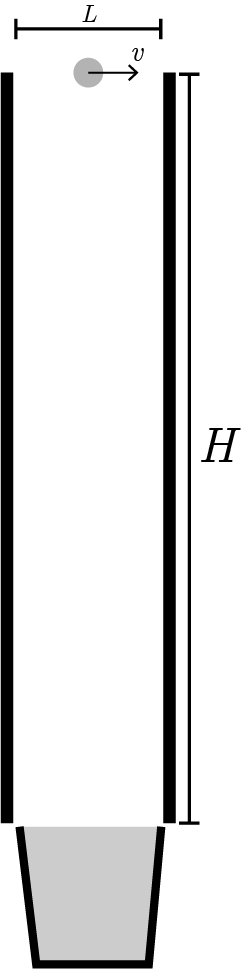
\includegraphics[height = 0.65\linewidth]{pr3.png}
\end{center}
\begin{choices}
    \item $1.2 \, \mathrm{m/s}$
    \item $2.0 \, \mathrm{m/s}$
    \item $2.3 \, \mathrm{m/s}$ \cor
    \item $3.5 \, \mathrm{m/s}$
    \item $4.6 \, \mathrm{m/s}$
\end{choices}
\end{prob}
\begin{sol}
    We use the reflection trick here, but we actually have to be a bit careful -- the radius is non-negligible! If we imagine that the radius is part of the walls, we see that the ping pong ball essentially bounces around between two boards which are separated by $L' = L - 2r = 0.16\,\unit m$. 
    
    This reduces to finding the minimum velocity such that the parabola that a point mass travels on crosses 7 boards separated by distance $L'$. that means that it travels a total distance $6.5L'$. Now it reduces to a standard kinematics problem. In the $y$-direction we have
    $$\frac 12 gt^2 = H \implies t = \sqrt{2H/g},$$
    and in the $x$-direction we have
    $$vt = 6.5L' \implies v = \frac{6.5L'}{\sqrt{2H/g}} = 2.3\,\unit{m/s}.$$
\end{sol}



\begin{prob}
    A bead of negligible size (not to scale in figure) is projected with speed $v$ on the inner wall of a spiral as shown. The radius of the spiral (i.e. the distance from the center to a point on the spiral) follows the relation $r=r_0(1/2)^{\theta/2\pi}$, where $\theta$ is the angle measured in radians from the initial radius $r_0$. 
    \begin{center}
        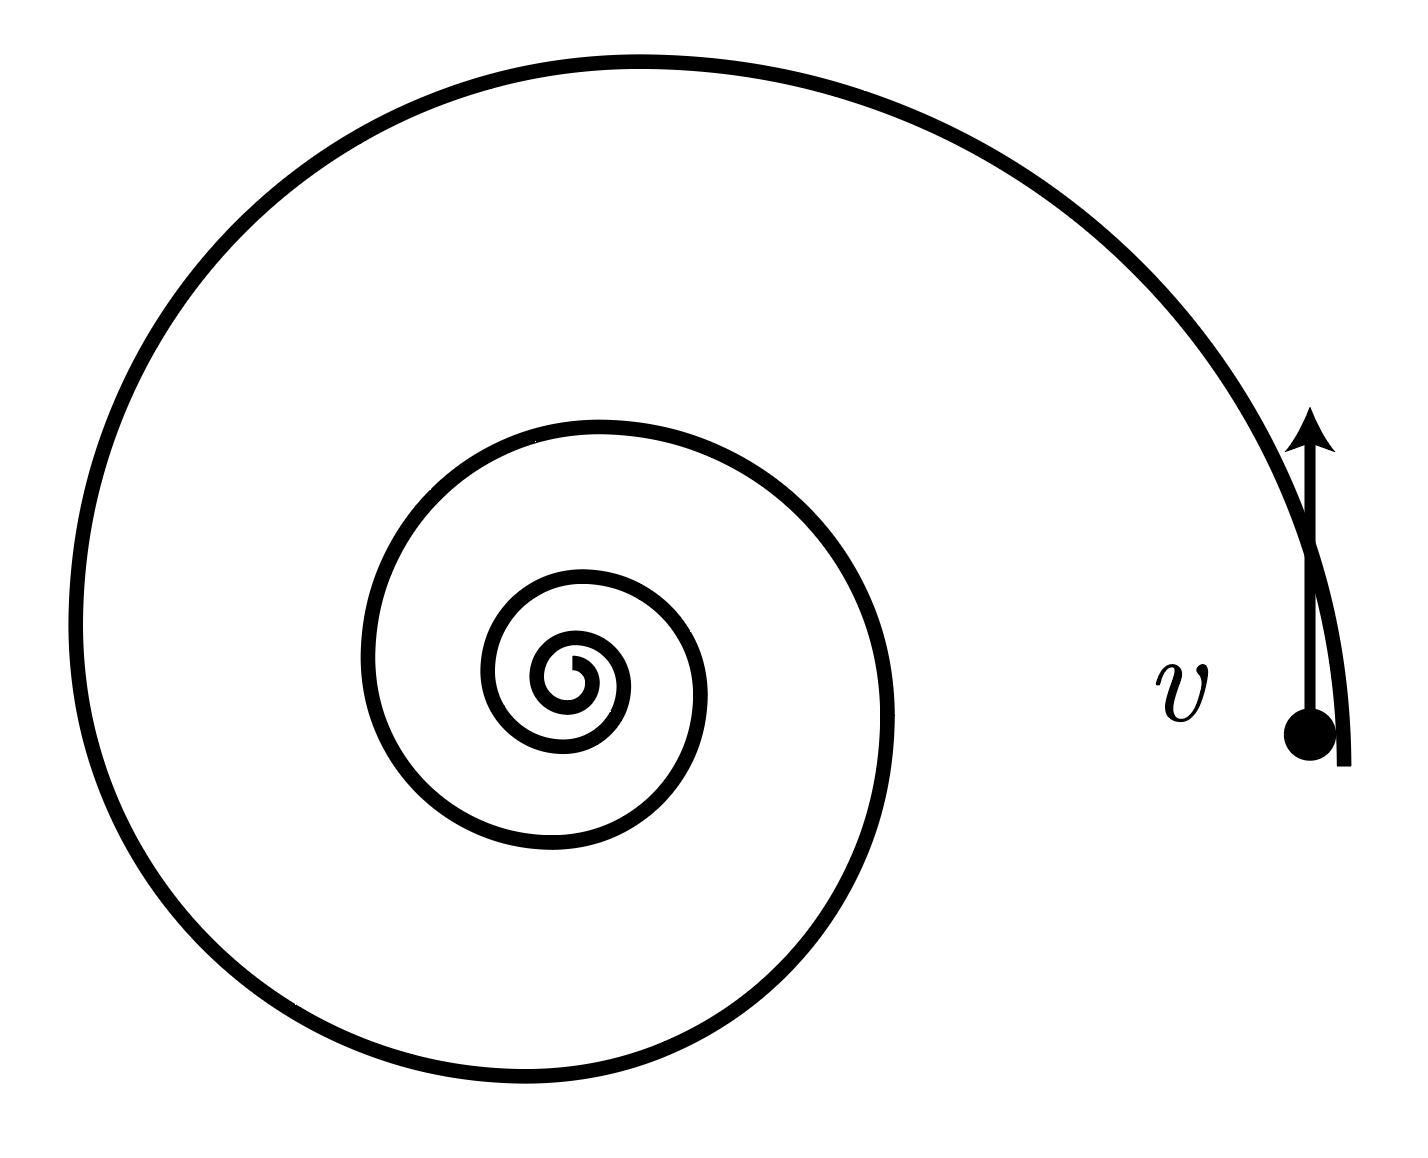
\includegraphics[scale=0.2]{spiral}
    \end{center}
    What graph shows the correct relation of $v$ as a function of time $t$?
    \begin{enumerate}[label = (\Alph*)]
\item 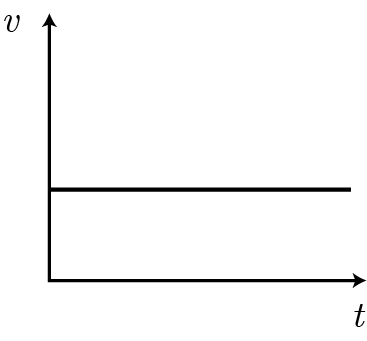
\includegraphics[scale=1]{an1} \textcolor{red}{$\leftarrow$ \textbf{CORRECT}}
\item 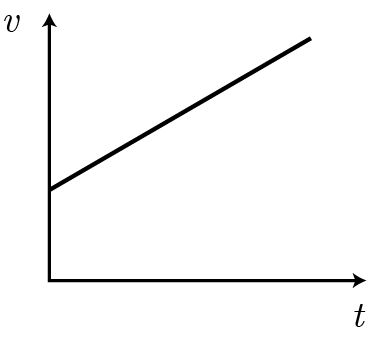
\includegraphics[scale=1]{an2}
\item 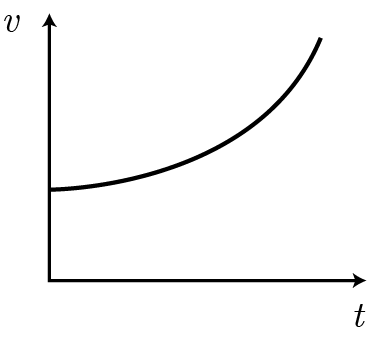
\includegraphics[scale=1]{an3}
\item 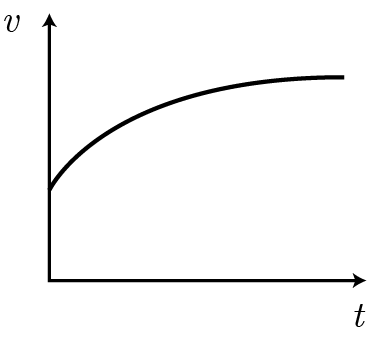
\includegraphics[scale=1]{an4}
\item 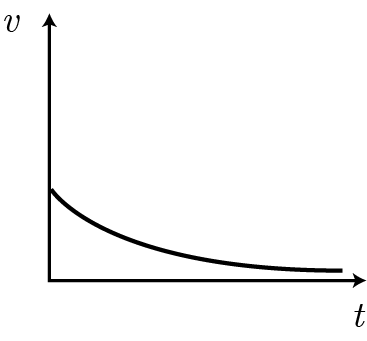
\includegraphics[scale=1]{an5}
\end{enumerate}
\end{prob}

\begin{sol}
    The spiral does no work on the bead, so the velocity stays constant.
\end{sol}

\begin{prob}
    A vertical hoop of radius $r$ is held in place with its bottom end on the ground. A small bead constrained to the hoop starts at the top of the hoop and is given a slight push. As the bead slides down the hoop, at what height $h$ above the ground is its vertical component of velocity the greatest?
\begin{enumerate}[label = (\Alph*)]
\item $r/6$  
\item $r/4$
\item $r/3$
\item $r/2$
\item $2r/3$ \textcolor{red}{$\leftarrow$ \textbf{CORRECT}}
\end{enumerate}
\end{prob}

\begin{sol}
    Let $\theta$ be the angle the bead has slid through along the hoop. By conservation of energy, its velocity at a given point is $v=\sqrt{2gr(1-\cos\theta)}$. As the bead slides, its vertical component of velocity will first increase, hit a maximum, and then decrease to 0 at the bottom of the hoop. Thus, we seek the point where the vertical acceleration of the bead is 0. The normal component of acceleration for the bead is given by $a_n=v^2/r=2g(1-\cos\theta)$ and the tangential component is simply $a_t=g\sin \theta$. To have their vertical components balance, we must have $$2(1-\cos\theta)(-\cos\theta)=\sin^2\theta.$$ Using the trigonometric identity $\sin^2\theta=1-\cos^2\theta$ and solving the quadratic, we get $\cos\theta = -1/3$. Hence, the point must be a height $h=r(1+\cos\theta)=2r/3$ above the ground.
\end{sol}

\begin{prob}
    A water sprinkler in the shape of a half-cylinder sprinkles water uniformly in all directions at velocity $v$ as shown. \begin{center}
        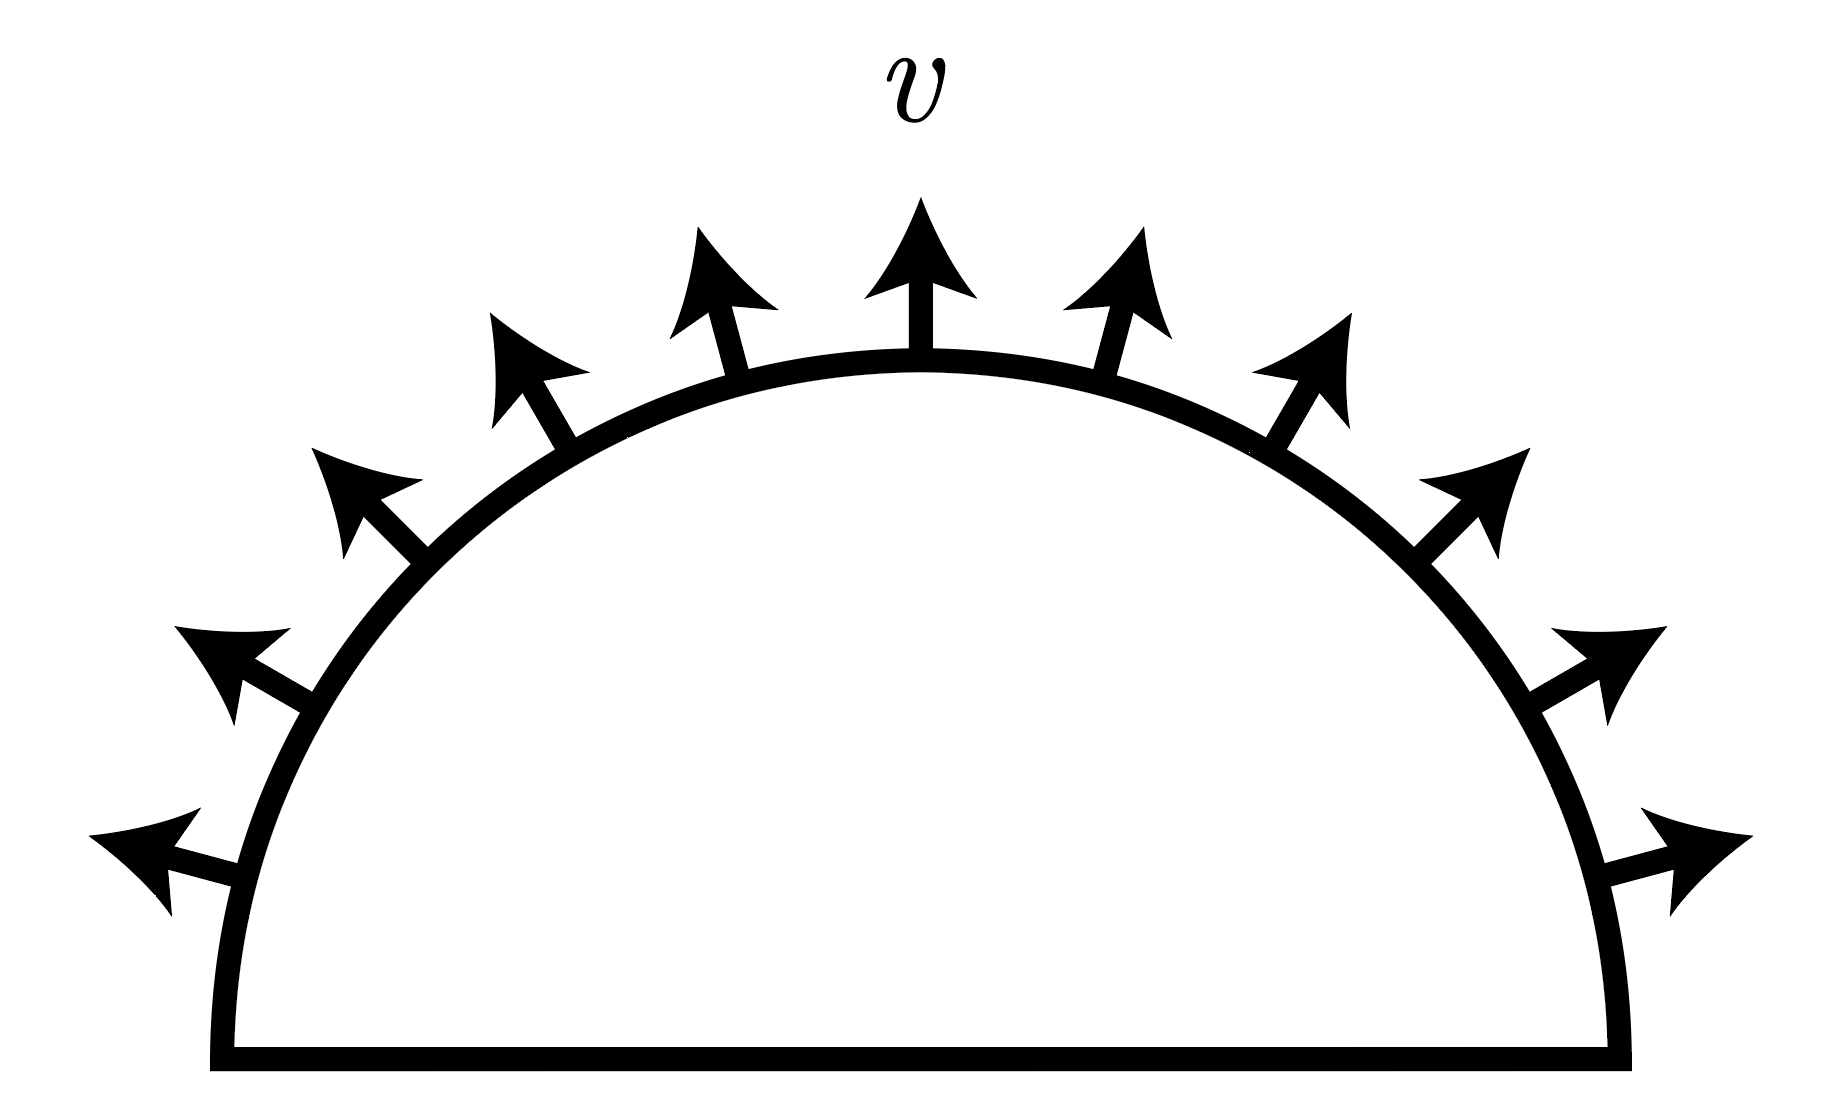
\includegraphics[scale=0.15]{sprinkler}
    \end{center}
    The sprinkler is placed flat on a lawn. At what horizontal distance $d$ from the sprinkler does the grass receive the most water per unit time?
    \begin{choices}
\item ${v^2}/{6g}$
\item ${v^2}/{4g}$
\item ${v^2}/{3g}$
\item ${v^2}/{2g}$
\item ${v^2}/{g}$ \textcolor{red}{$\leftarrow$ \textbf{CORRECT}}
\end{choices}
\end{prob}

\begin{sol}
    As a function of the angle $\theta$ at which the water is sprinkled, the distance the water travels follows $$d=\frac{v^2\sin 2\theta}{g}$$Note that for water sprayed out between angles $\theta$ and $\theta+\Delta \theta$, what matters is the width of the strip of grass in which the water lands, i.e. between $d$ and $d+\Delta d$. The smaller this width, the greater the density of water landing at a given point. Since the water sprayed above $45^\circ$ is symmetric to that below, we only need to analyze $\theta$ up to $45^\circ$. Notice that since $d\propto \sin 2\theta$, $\Delta d$ is smallest when  $\Delta \sin2\theta$ is smallest (i.e. when the slope of $\sin2\theta$ is smallest). This clearly occurs at $\theta=45^\circ$, and evaluating $d$ at this angle $\theta$ yields $d=v^2/g$. 
\end{sol}

\begin{prob}
    A non-Hookian spring with constant $k$, when stretched by a distance $x$, has potential energy $$U=\frac12kx^{8/5}.$$ A mass $m$ is connected to the spring and at equilibrium is given a speed $v_0$, which results in oscillations of frequency $\omega_0$. What is the new frequency of oscillation if the mass is instead given a speed $16v_0$ at equilibrium?
    \begin{enumerate}[label = (\Alph*)]
\item $\omega_0$
\item $\omega_0/2$ \textcolor{red}{$\leftarrow$ \textbf{CORRECT}}
\item $\omega_0/4$
\item $\omega_0/16$
\item $\omega_0/32$
\end{enumerate}
\end{prob}

\begin{sol}
    By conservation of energy, the velocity $v^2\propto x^{8/5}\Rightarrow v^{5/4}\propto x$. Now, the frequency is given by $\omega\propto v/x\propto v^{-1/4}$. Thus, if we multiply $v$ by 16, $\omega$ is halved.
\end{sol}

\begin{prob}
    A small hollow cylinder of mass $m$ and radius $r$ can roll without slipping along the inside of a fixed hollow cylinder of radius $R$. If the small cylinder starts off at only a slight offset to the bottom of the larger cylinder, it will exhibit simple harmonic oscillations with frequency $\omega$. Find $\omega$. 
    \begin{enumerate}[label = (\Alph*)]
\item $\sqrt{g/R}$
\item $\sqrt{g/2R}$ \textcolor{red}{$\leftarrow$ \textbf{CORRECT}}
\item $\sqrt{g/r}$
\item $\sqrt{g/2r}$
\item $\sqrt{gr/R^2}$
\end{enumerate}
\end{prob}

\begin{sol}
    Let $\theta\ll 1$ be the angular position of the small cylinder within the larger one. At this point, the small cylinder is effectively on a slope of angle $\theta$. Taking torque about the point of contact with the larger cylinder and using the parallel axis theorem with $I=2mr^2$, we get the linear acceleration $a=g/2$. As a result, $\ddot \theta=-(g/2R)\theta$, so $\omega=\sqrt{g/2R}$.
\end{sol}

\textbf{The following information applies to Problems \ref{cylin1} and \ref{cylin2}.}\\
Anna is rolling a cylinder of snow on the ground. At the start, the cylinder has mass $m$ and radius $r$. Assume the cylinder has uniform density. Anna begins rolling the cylinder without slipping along the ground, which has a dusting of snow with linear mass density $\lambda$. Assume that as the cylinder rolls, its density stays constant, and assume $\lambda \ll m/r$. There is no energy loss to friction or other dissipating forces.

\begin{prob}\label{cylin1}
    Anna gently rolls the cylinder at a constant speed $v\ll \sqrt{gr}$. Assume she always pushes at the cylinder's center, parallel to the ground. Over the course of one revolution, how must her force exerted on the cylinder change with respect to time? Note: the value of $F$ at the $t$ axis may not be 0 and can vary between graphs.
    \begin{enumerate}[label = (\Alph*)]
\item 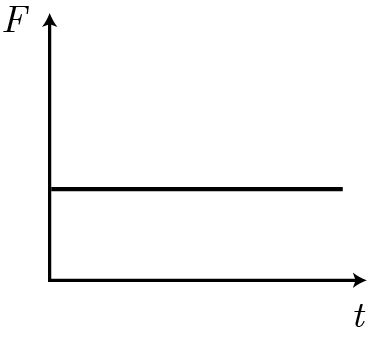
\includegraphics[scale=1]{ans1}
\item 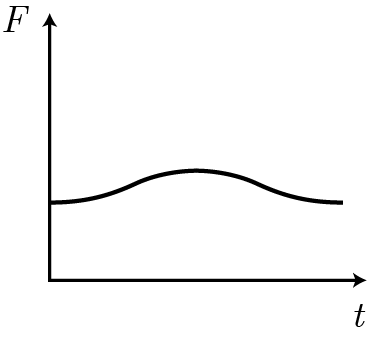
\includegraphics[scale=1]{ans2.png} \textcolor{red}{$\leftarrow$ \textbf{CORRECT}}
\item 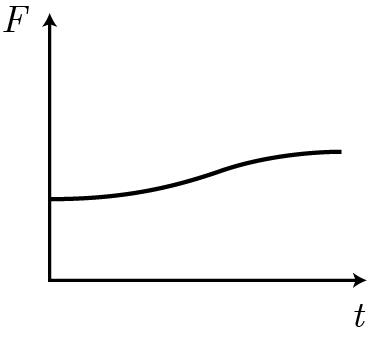
\includegraphics[scale=1]{ans3.png}
\item 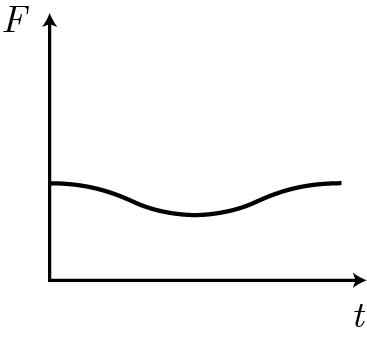
\includegraphics[scale=1]{ans4.png}
\item 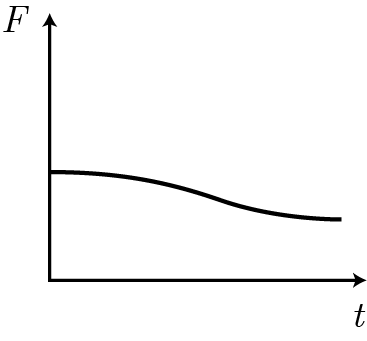
\includegraphics[scale=1]{ans5.png}
\end{enumerate}
\end{prob}

\begin{sol}
    As the cylinder picks up snow, there will be an excess of mass on the back side of the cylinder that will cause gravity to exert a torque backwards. As this mass accumulates, the force Anna needs to exert increases until we reach half a revolution, at which point mass will begin to accumulate on the other side of the cylinder, causing a restoring torque the other way. Thus, by the end of one revolution the required force decreases back to its original state. 
\end{sol}

\begin{prob}\label{cylin2}
    Find the average force exerted by Anna over one revolution, i.e. the average value of the curve you found in the previous problem.
    \begin{enumerate}[label = (\Alph*)]
\item $\lambda gr$ \textcolor{red}{$\leftarrow$ \textbf{CORRECT}}
\item $2\pi \lambda gr$
\item $\lambda v^2/g$
\item $\lambda v^2/2\pi g$
\item $\lambda^2r v^2/2\pi mg$
\end{enumerate}
\end{prob}

\begin{sol}
    The work that Anna does is $2\pi rF$, and the increase in energy of the system belongs in the increased potential energy of the picked up snow, which is $(2\pi r\lambda)gr$. Equating these quantities yields $F=\lambda gr$. 
\end{sol}

\begin{prob}
    A system of $2N$ identical gears with mass $m$ and radius $r$ are connected to each other in a line as shown. The gears can be assumed to act as uniform cylinders, with the ``teeth" having negligible mass. 
    \begin{center}
        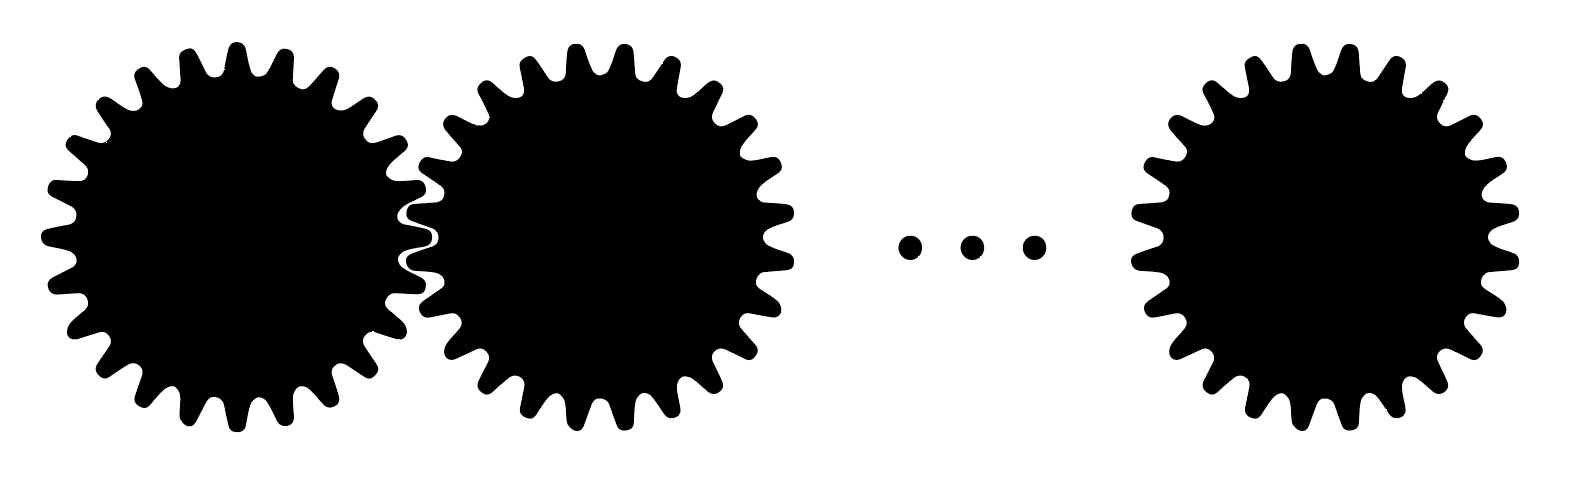
\includegraphics[scale=0.2]{gears}
    \end{center}
    A torque $\tau$ is applied to the rim of the $N$th gear from the left to accelerate it at angular acceleration $\alpha$. What is the necessary value of $\tau$?
    \begin{enumerate}[label = (\Alph*)]
\item $mr^2\alpha/4N$
\item $Nmr^2\alpha/2$
\item $Nmr^2\alpha$ \textcolor{red}{$\leftarrow$ \textbf{CORRECT}}
\item $\frac{N-1}{N+1}mr^2\alpha$
\item $\frac{N}{N+1}mr^2\alpha$
\end{enumerate}
\end{prob}

\begin{sol}
    Let the gears pick up some angular velocity $\omega$ after spinning an angle $\theta$. The work done by torque is $\tau\theta$, and this equals the kinetic energy $(2N)(1/2)(mr^2/2)\omega^2$. By the kinematic formula, $\alpha=\omega^2/2\theta$ so $$\tau=Nmr^2\frac{\omega^2}{2\theta}=Nmr^2\alpha$$
\end{sol}

\textbf{The following information applies to Problems \ref{block1} and \ref{block2}.}\\
Two identical blocks of mass $m$ are stacked on top of one another on a plane of incline $\theta$. The coefficient of friction between the blocks and between the blocks and the plane is $\mu<\tan\theta$. You seek to apply the smallest possible force $F$ to either one of the blocks, parallel to the plane, in order to keep the setup in static equilibrium.

\begin{prob}\label{block1}
    You hypothesize that for some values of $\mu$, no possible force $F$ exists. What range of values for $\mu$ make it impossible to find a force $F$ to keep the setup in static equilibrium?
    \begin{enumerate}[label = (\Alph*)]
\item $0<\mu<(\tan\theta)/6$
\item $0<\mu<(\tan\theta)/4$
\item $0<\mu<(\tan\theta)/3$ \textcolor{red}{$\leftarrow$ \textbf{CORRECT}}
\item $0<\mu<(\tan\theta)/2$
\item All values of $\mu<\tan\theta$ will yield a possible $F$.
\end{enumerate}
\end{prob}

\begin{sol}
    Clearly we need to exert $F$ on the top block, or otherwise the top block will just slide. The worst-case scenario for the bottom block is then with gravity pulling downwards and with friction on both of its faces pointing upwards. This yields $mg\sin\theta=mg\mu\cos\theta+2mg\mu\cos\theta\Rightarrow \mu=(\tan\theta)/3$. Any $\mu$ less than this will fail. 
\end{sol}

\begin{prob}\label{block2}
    Assuming that $\mu$ is at the lowest possible value to allow a solution to $F$, what is $F$?
    \begin{enumerate}[label = (\Alph*)]
\item 0
\item $(1/2)mg\sin\theta$
\item $mg\sin\theta$
\item $(4/3)mg\sin\theta$ \textcolor{red}{$\leftarrow$ \textbf{CORRECT}}
\item $(3/2)mg\sin\theta$
\end{enumerate}
\end{prob}

\begin{sol}
    At this critical case, our condition for equilibrium on the bottom block is satisfied. Now, analyzing the top block, friction of magnitude $mg\mu\cos\theta=(mg\sin\theta)/3$ points downward as well as the gravitational $mg\sin\theta$. The total force that thus needs to be balanced by $F$ is $(4/3)mg\sin\theta$. 
\end{sol}

\begin{prob}
    A bead of mass $m$ is bouncing elastically at speed $v$ inside a uniform hollow cube of mass $M$ and side length $L$. The cube is free to move on the floor. Assume all surfaces are frictionless and that the center of mass of the system is at rest. In the lab frame, what is the horizontal range of the bead's motion?
    \begin{enumerate}[label = (\Alph*)]
\item ${mL}/(m+M)$ 
\item ${2mL}/(m+M)$
\item ${ML}/(m+M)$ \textcolor{red}{$\leftarrow$ \textbf{CORRECT}}
\item ${2ML}/({m+M})$
\item ${(m+M)L}/{m}$
\end{enumerate}
\end{prob}

\begin{sol}
    At the point where the bead is at one of the cube's walls, its distance from the center of mass of the cube is $L/2$. Its distance from the total center of mass of the system is thus $(L/2)M/(m+M)$. The total range of motion oscillates symmetrically about the system center of mass, so the answer is just double this. 
\end{sol}

\begin{prob}
    A car windshield of area $A$ makes an angle $\theta$ with the horizontal as it drives through the rain. The rain falls at a constant speed $v_0$ downward while the car drives through it horizontally at speed $u_0$. If the rain droplets have number density $n$, how many rain droplets hit the windshield per unit time?
    \begin{choices}
        \item $(u_0+v_0)An\cos \theta$
        \item $(u_0 + v_0)An \sin \theta$
        \item $u_0An \cos \theta + v_0An\sin\theta$ \cor
        \item $u_0An\sin \theta + v_0An \cos \theta$
        \item $\sqrt{u_0^2 + v_0^2} An\tan\theta$
    \end{choices}
\end{prob}
\begin{sol}
    Working in the frame of the rain, we see that the rate of droplets encountered is given by
    $$nAv_\perp,$$
    where $v_\perp$ is the component of the velocity perpendicular to the windshield. In the frame of the rain, the velocity of the windshield is
    $$v_0 \hat x + u_0 \hat y,$$
    so the perpendicular component is 
    $$v_0\sin \theta + u_0\cos \theta,$$
    which means that our total rate is
    $$\frac{dN}{dt} = nA(v_0\sin \theta + u_0\cos \theta) = u_0An \cos \theta + v_0An\sin\theta.$$
\end{sol}

\begin{prob}
    Playing cornhole, Collin attempts to land his beanbag within a circle of radius $r$ a distance $d \gg r$ away. Assuming that he throws at the correct velocity, what is the maximum possible error in his throwing angle $\delta \theta$ for him to land it within the circle in terms of $d$ and $\theta$?
    \begin{choices}
        \item $\frac{rg}{2v^2\cos (2\theta)}$ \cor
        \item $\frac{rg}{v^2 \cos (2\theta)}$
        \item $\frac{rg}{2v^2\sin (2\theta)}$
        \item $\frac{rg}{v^2\sin(2\theta)}$
        \item $\frac{rg}{2v^2\tan(2\theta)}$
    \end{choices}
\end{prob}
\begin{sol}
    The range as a function of $v$ and $\theta$ is
    $$d = \frac{v^2 \sin (2\theta)}{g},$$
    so we have by error propagation
    $$\delta d = \frac{2v^2 \cos (2\theta)}{g} \delta \theta.$$
    And for it to land with in the radius $r$ cornhole, we should have $\delta d = r$, so
    $$\delta \theta = \frac{g}{2v^2\cos(2\theta)} r.$$
\end{sol}

\begin{prob}
    In the setup below, two massless strings hold up both a table of mass $M$ and two masses of mass $m$. The table and the masses are only attached to each other via the two strings which are hooked on the ceiling, and the string makes an angle $\theta$ with where it attaches to the table while attaching directly vertically to the masses. What is the minimum mass $m$ such that the setup remains static?
    \begin{center}
        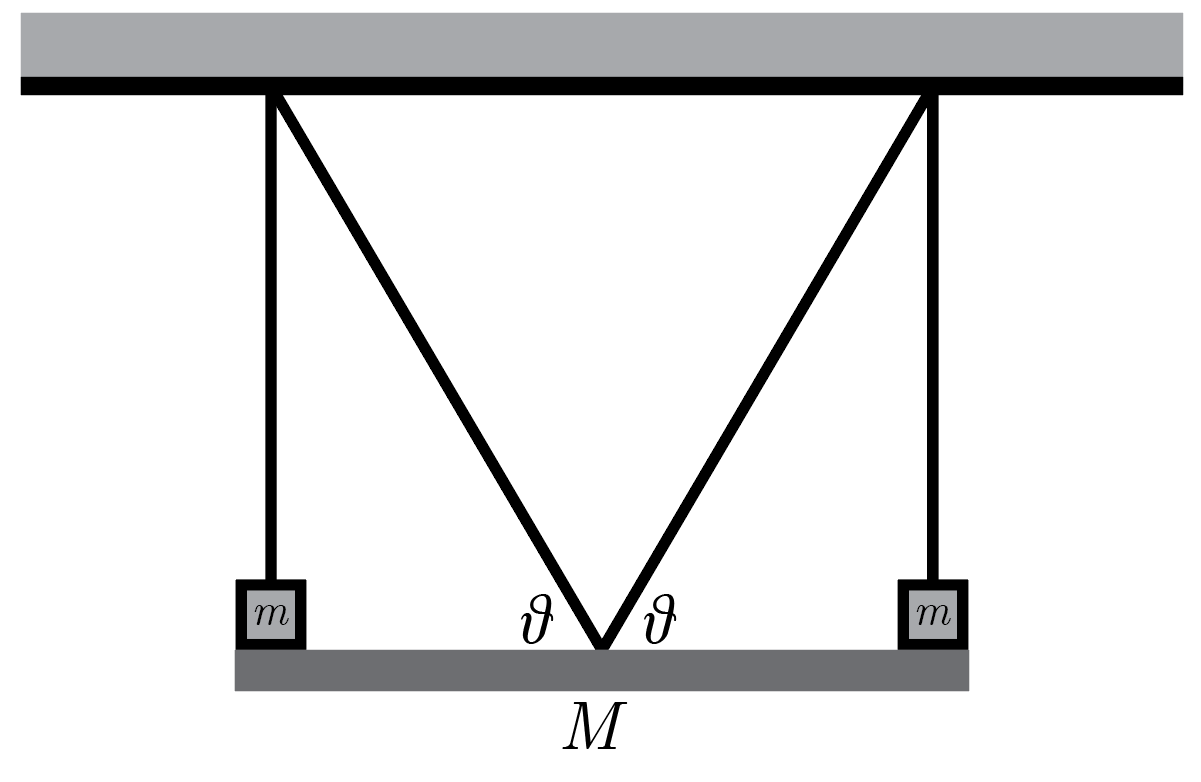
\includegraphics[width=6cm]{table_masses.png}
    \end{center}
    \begin{choices}
        \item $\frac{M\cos \theta}{2}$
        \item $\frac{M}{2\cos \theta}$
        \item $\frac{M\sin \theta}{2}$
        \item $\frac{M}{2\sin \theta}$ \cor
        \item $\frac{M}{\sin \theta + \cos \theta}$
    \end{choices}    
\end{prob}
\begin{sol}
    In the minimum case, the normal force between the masses $m$ and the table should be $0$. Thus, the tension in the string is $mg$, which means that balancing forces on the tab le we have
    $$Mg = 2mg \sin \theta \implies m = \frac{M}{2\sin \theta}.$$
\end{sol}

\begin{prob}
    Justin is gardening his plants with a hose with length $l$ and radius $r$ that takes in water at pressure $P_0$. The flow is in the viscous regime with coefficient $\eta$. If he switches out his hose for one of radius $2r$, by what factor does his volume flow rate change?
    \begin{choices}
        \item $\sqrt 2$
        \item $2$
        \item $2^2$
        \item $2^3$
        \item $2^4$ \cor
    \end{choices}
\end{prob}
\begin{sol}
    We use some proportional reasoning using general facts that we know about the terms given in the equation. This is not completely dimensional analysis, but it is a similar mode of reasoning. We know that we can write force in two different ways:
    \begin{align*}
        F &= PA,\\
        F &= \eta A \frac{v}{y}.
    \end{align*}
    We can imagine those two are opposing in this case, so we write
    $$P(r^2) \sim \eta (rl) \frac{v}{r}.$$
    This gives us that the speed of the water is on the order of $v \sim Pr^2/l$. And volume flow rate is proportional to $vA$, so we can write $Q \sim \frac{Pr^2}{l}r^2$, so $Q \propto r^4$, giving us choice $E$.
\end{sol}

\begin{prob}
    A hoop of mass $M$ and radius $R$ is placed on a peg of radius $r < R$. It is then nudged slightly and the hoop begins oscillating while remaining in contact with the peg at all times. What is the angular frequency of oscillation?
    \begin{choices}
        \item $\sqrt{\frac{g(R-r)}{2R^2 -2Rr + r^2}}$ \cor
                \item $\sqrt{\frac{gR}{2(R^2 + r^2)}}$
        \item $\sqrt{\frac{gr}{R^2 + 2Rr + r^2}}$
        \item $\sqrt{\frac{g(R-r)}{R^2 - 2Rr + r^2}}$
        \item $\sqrt{\frac{g}{R^2 +2Rr + 2r^2}}$
    \end{choices}
\end{prob}
\begin{sol}
    Because the outer ring and the hoop remain tangent at all times, we can connect their two centers. This clearly shows that the motion is equivalent to the hoop oscillating while pivoted a distance $R-r$ away from its center! Thus, we can use our normal technique of finding the oscillation period of a physical pendulum. The distance of the COM from the pivot point is $d = R-r$ and the moment of inertia is
    $$I = MR^2 + Md^2 = M(2R^2 -2Rr +r^2).$$
    Our equation of motion becomes
    $$I \ddot \theta = - mg(R-r) \theta \implies \omega = \sqrt{\frac{mgd}{I}} = \sqrt{\frac{g(R-r)}{2R^2 -2Rr + r^2}}.$$
\end{sol}

\textbf{The following information applies to Problems \ref{pull1} and \ref{pull2}.}\\
Matthew is pulling on a chord by moving his hand in a circle. The chord is hinged at point $A$, his hand is at point $H$ and his elbow remains fixed at point $E$. His arm has length $EH = \ell$ and the hinge-point is a distance $AE = d > \ell$ away.
\begin{center}
    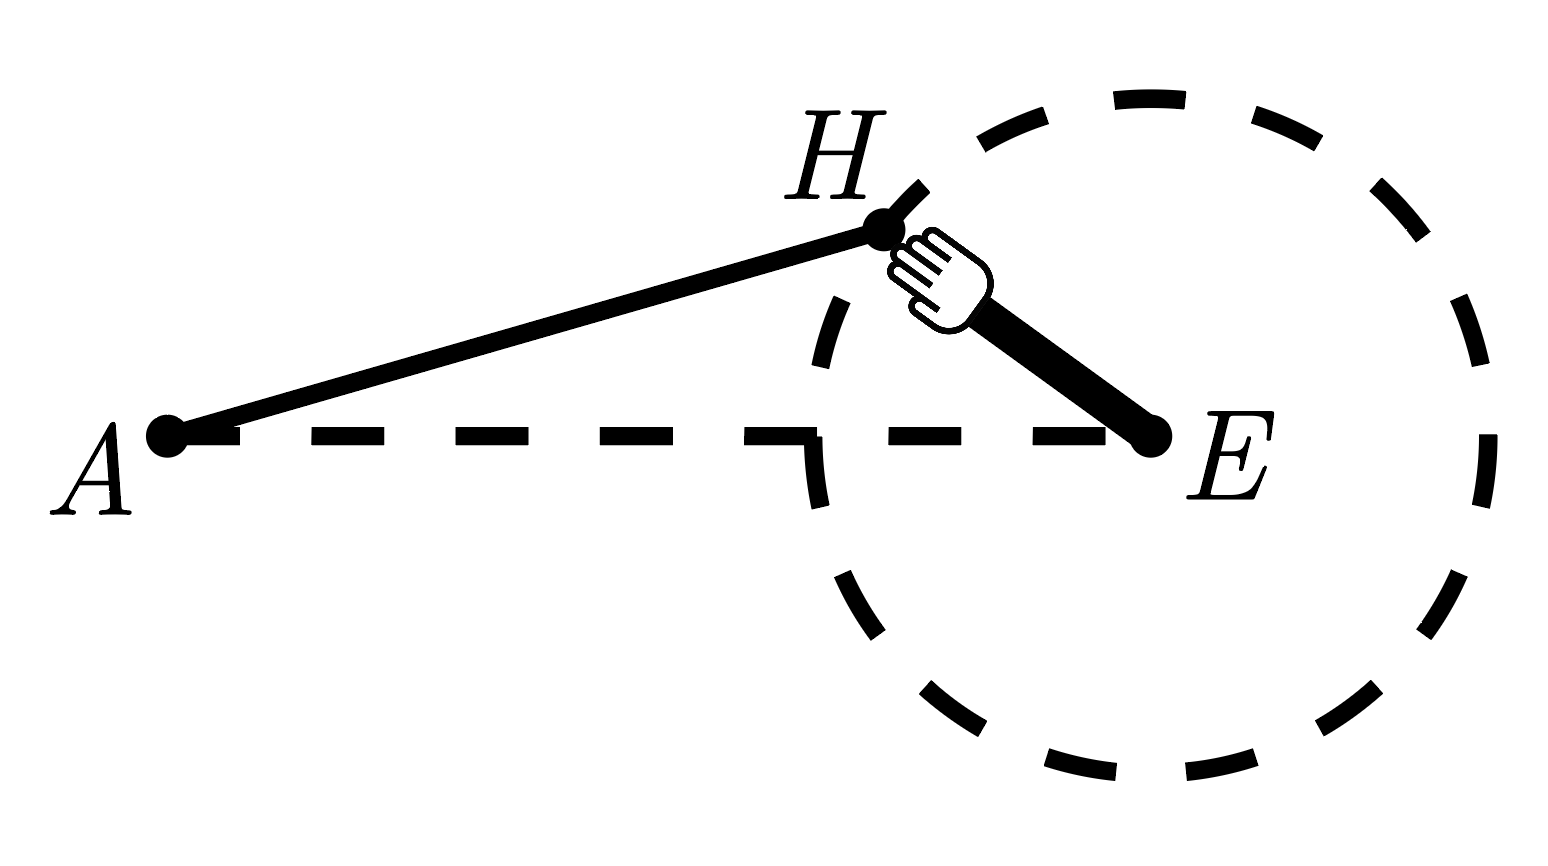
\includegraphics[width=7cm]{pull.png}
\end{center}

\begin{prob}\label{pull1}
    Suppose that the chord has constant tension $T$ as it is pulled. At what angle from the horizontal does Matthew experience maximum torque?
    \begin{choices}
        \item $\sin^{-1}(\ell/d)$
        \item $\cos^{-1}(\ell/d)$ \cor
        \item $\tan^{-1}(\ell/d)$
        \item $\pi/4$
        \item $\pi/2$
    \end{choices}
\end{prob}

\begin{sol}
    Because it is constant tension, the torque is maximized when the moment arm is largest. This is when the two lines $AH$ and $HE$ are perpendicular. Thus, we have a right triangle $\triangle AHE$, and so
    $$\cos \theta = \frac{HE}{AE} = \frac{\ell}{d} \implies \theta = \cos^{-1} (\ell/d).$$
\end{sol}


\begin{prob}\label{pull2}
    Suppose now that the chord of constant tension is replaced with a zero length spring which is fixed at point $A$ with spring constant $k$. At what angle from the horizontal does Matthew experience maximum torque?
    \begin{choices}
        \item $\sin^{-1}(\ell/d)$
        \item $\cos^{-1}(\ell/d)$
        \item $\tan^{-1}(\ell/d)$
        \item $\pi/4$
        \item $\pi/2$ \cor
    \end{choices}
\end{prob}
\begin{sol}
    We have that the torque in this case is
    $$\tau = (kAH) HE \sin \angle AHE = 2k [AHE].$$
    The area of the triangle is maximized when $\overline {AE} \perp \overline {HE}$, so we get $E$.
\end{sol}

\textbf{The following information applies to Problems \ref{roll1} and \ref{roll2}.}\\
David launches a uniform sphere of mass $M$ and radius $r$ down an inclined plane which has coefficient of friction $\mu$, and inclination angle $\theta$ with velocity $v_0$.

\begin{prob}\label{roll1}
    What is the condition on $\theta$ such that the uniform sphere eventually begins rolling without slipping?
    \begin{choices}
        \item $\tan \theta < \frac 57 
        \mu$
        \item $\cot \theta < \frac 57 \mu$
        \item $\tan \theta < \frac 72 \mu$ \cor
        \item $\cot \theta > \frac 27 \mu$
        \item $\tan \theta < \frac 52 \mu$
    \end{choices}
\end{prob}
\begin{sol}
    We write the force and torque equations on the sphere:
    \begin{align*}
        ma &= mg\sin \theta - \mu mg \cos \theta, \\
        \frac 25 mR^2 \alpha &= \mu mg \cos \theta R.
    \end{align*}
    So, using this we can write $\omega(t)$ and $v(t)$:
    \begin{align*}
        \omega(t) &= \frac 52 \frac{\mu g \cos \theta}{R}t,\\
        v(t) &= v_0 + (g\sin \theta - \mu g \cos \theta) t.
    \end{align*}
    So, if it ever begins rolling without slipping we must have some $t> 0 $ such that $\omega(t) R  = v(t)$,
    \begin{align*}
        &\frac 52 \mu g \cos \theta t = v_0 + (g\sin \theta - \mu g \cos \theta)t\\
        &\left(\frac 72 \mu g \cos \theta - g\sin \theta\right) t = v_0.
    \end{align*}
    Thus, a solution exists if $\frac 72 \mu g \cos \theta - g \sin \theta > 0 \implies \tan \theta < \frac 72 \mu$.
\end{sol}

\begin{prob}\label{roll2}
    Assuming that $\theta$ satisfies the condition found in problem \ref{roll1}, how long does it take for the sphere to begin rolling without slipping?
    \begin{choices}
        \item $\frac{v_0}{\frac 72 \mu g \cos \theta - \frac 52g\sin \theta}$
        \item $\frac{v_0}{ \mu g \cos \theta - \frac 52 g\sin \theta}$
        \item $\frac{v_0}{\frac 52 \mu g \cos \theta - g\sin \theta}$
        \item $\frac{v_0}{\frac 72 \mu g \cos \theta - g\sin \theta}$ \cor
        \item $\frac{v_0}{ \mu g \cos \theta - \frac 72 g\sin \theta}$
    \end{choices}
\end{prob}
\begin{sol}
    For this part, we simply work off of the last equation we found in problem 22, which gives us 
    $$t = \frac{v_0}{\frac 72  \mu g \cos \theta - g\sin \theta}.$$
\end{sol}

\begin{prob}
A rectangular container has four mass-less walls of width $w$ and height $h$. Two of the walls are adjustable, that is to say, the width in one dimension can be reduced. The water holds a volume $V$ of water. Find the maximum force $F$ that can be applied on the adjustable walls before water comes out of the top of the container. Take water's density as $\rho$.
\begin{center}
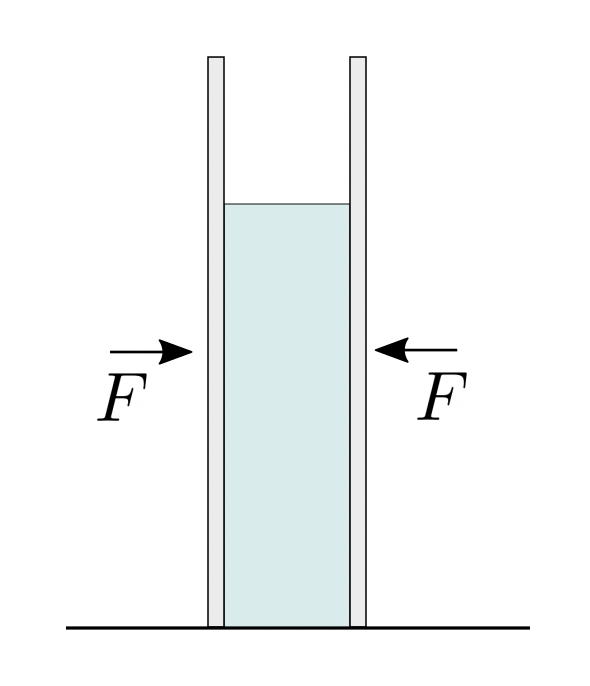
\includegraphics[width = 0.3\linewidth]{pr17}
\end{center}
\begin{choices}
\item $\frac{1}{2} \rho g w h^2$ \cor
\item $\frac{1}{2} \rho g w^2 h$
\item $\rho g V$
\item $\rho g w h^2$
\item $\rho g w^2 h$
\end{choices}
\end{prob}
\begin{sol}
    The average gauge pressure on the wall is $P_{\text{avg}} = \rho g \frac h2$, so the total force on the wall is,
    $$F = P_{\text{avg}}A = P_{\text{avg}} wh = \frac 12 \rho g w h^2.$$
\end{sol}

\begin{prob}
    Ne just built a half-cylindrical sail and wants to test it for tearing. It has a radius $r$ and depth $d$. Air comes in at a velocity $v$ and density $\rho$. Assume unrealistically that when the air hits the sail, it loses all of its velocity. What is the average pressure experienced by the sail?
    \begin{center}
        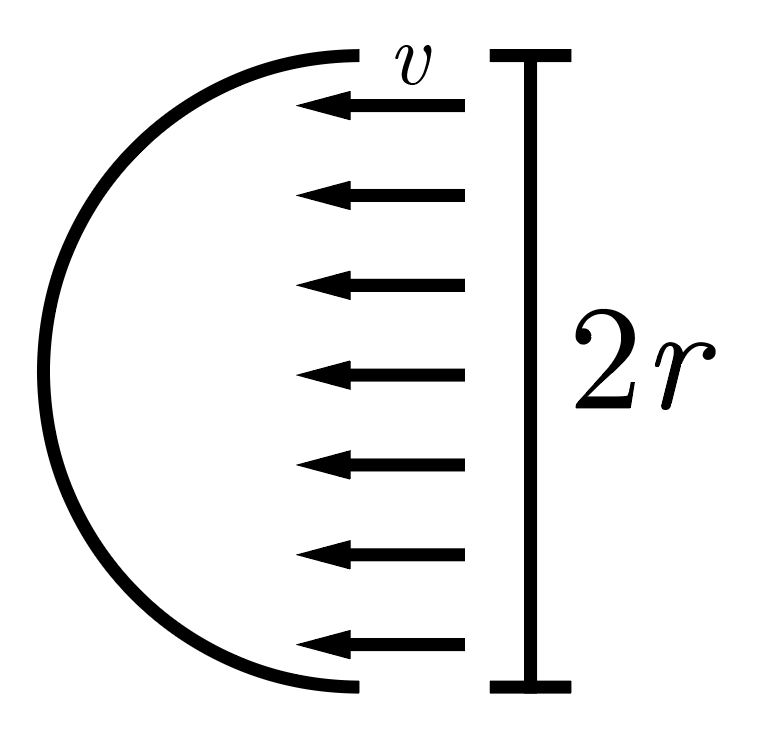
\includegraphics[width=5cm]{cylinder_sail.png}
    \end{center}
    \begin{choices}
        \item $\frac{2\rho v^2}{\pi}$. \cor
        \item $\frac{\pi \rho v^2}{2}$
        \item $\rho v^2$
        \item $\frac{\rho v^2}{\pi}$
        \item $\pi \rho v^2$
    \end{choices}
\end{prob}

\begin{sol}
    We want to add up the total magnitude of force on all the pieces of the half-cylinder. At a piece $\theta$ from the vertical, the magnitude of the force experienced is 
    $$F = \rho(d A \sin \theta) v^2.$$
    This means we can project this down onto the rectangle, and thus the sum of the magnitudes of the force experienced is
    $$\sum F = \rho v^2 (2r)d.$$
    Thus, the average pressure is $\sum F / A = 2rd \rho v^2 / (\pi r d) = 2\rho v^2/\pi$.
\end{sol}



\end{document}